\documentclass[../main.tex]{subfiles}

\setstretch{0.1} % 

\begin{document}

\chapter{Introduction}
\begin{floatingfigure}[r]{0.3\textwidth}%
    \vspace{\dimexpr0.3\baselineskip-\topskip}%
    \noindent
    \includegraphics[width=0.3\textwidth]{Images/Introduction/optical_flat}
    \caption{Example of an optical flat. \cite{optical_flat_mitutoyo}}
    \label{fig:optical_flat_example}
\end{floatingfigure}
Optical flats are precision devices used in the field of material science to measure the flatness of surfaces or to create precisely flat surfaces. An optical flat is typically a high-quality, polished, flat glass or quartz disc used in conjunction with monochromatic light to form interference fringes that can be observed and measured to assess surface flatness or quality.\footnote{Optical flats should be handled with great precaution as they are very fragile.} \cite{Toru_2017, edmund_optics_optical_flats, kemet_optical_flats, lapmaster_wolters_optical_flats,Paschottaoptical_flats}
% \begin{frame}{}
%     \begin{figure}[h]
%         \centering
%         \includegraphics[width=0.8\textwidth]{Images/Introduction/optical_flat}
%         \caption{Example of an optical flat. \cite{optical_flat_mitutoyo}}
%         \label{fig:optical_flat_example}
%     \end{figure}
% \end{frame}
\section{Physical Characteristics}
\setstretch{4}
\subsection{Material Composition}
\setstretch{0.1} % 
Optical flats are predominantly made from two types of materials: fused silica and ultra-low expansion (ULE) glass. Fused silica, known for its exceptional optical clarity and thermal stability, is ideal for precision measurement tools. It has a very low coefficient of thermal expansion, which means it remains stable under varying temperatures, thereby minimizing measurement errors due to thermal variations (figure \ref{fig:refractive_index_silica}).\cite{Paschottafused_silica}


% \begin{wrapfigure}{r}{0.4\textwidth}
%     \centering
%     \includegraphics[width=0.4\textwidth]{Images/Introduction/silica_refractive_index}
%     \caption{The refractive index of fused silica versus wavelength at three different temperatures. \cite{Paschottafused_silica}}
%     \label{fig:refractive_index_silica}
% \end{wrapfigure}

Ultra-low expansion glass, such as Corning's ULE glass, is another favored material. This glass type is engineered to have extremely low thermal expansion rates, which are crucial in maintaining the accuracy of measurements in environments with fluctuating temperatures. ULE glass's robustness and resistance to thermal stress make it particularly suitable for high-precision optical applications, including astronomy and semiconductor manufacturing.\cite{Corning_2022}

Both materials are chosen not only for their minimal thermal properties but also for their ability to be polished to high optical qualities, ensuring that the optical flat does not introduce aberrations or distortions in the interference patterns used for surface measurements.\cite{Corning_2022,Paschottafused_silica,doi:https://doi.org/10.1002/9780470135976.ch1}
\begin{figure}[H]
    \centering
    \includegraphics[width=0.8\textwidth]{Images/Introduction/silica_refractive_index}
    \caption{The refractive index of fused silica versus wavelength at three different temperatures. \cite{Paschottafused_silica}}
    \label{fig:refractive_index_silica}
\end{figure}
\subsection{Surface Quality}
The surface of an optical flat is meticulously polished to achieve a high degree of flatness, typically within fractions of a wavelength of light (\(\lambda/20\) or better). This extreme flatness is crucial for the accuracy of optical measurements. Any imperfections on the surface can distort the interference fringes, leading directly to measurement errors.\cite{enwiki:1212101911}

After the initial polishing phases, optical flats may undergo additional processing steps such as the application of dielectric coatings. These enhancements are critical when the optical flats are used as reference mirrors in precision instruments like the Twyman–Green interferometer, where the utmost flatness is crucial.\cite{Paschottaoptical_flats}

The final quality of optical flats is often verified in an interferometric setup, where they are compared against a reference surface that is of even higher precision. Occasionally, these reference surfaces may utilize fluids like mercury to achieve near-perfect flatness levels, although such materials are challenging to handle and maintain.\cite{Paschottaoptical_flats}

\section{Working Principle}
The principle behind optical flats relies on the optical phenomenon of interference. This section delves into how interference fringes are formed, their types, and their importance in measuring surface characteristics.

\subsection{Interference Fringes}
Interference fringes are the result of the wave nature of light. When monochromatic light—light of a single wavelength—is used to illuminate the interface between an optical flat and another surface, variations in the gap created by surface irregularities cause the waves of light to overlap and interfere with each other. This interference can constructively or destructively affect the light waves, resulting in a pattern of dark and light bands known as interference fringes, which can be observed and analyzed.

\subsubsection{Formation of Fringes}
\begin{floatingfigure}[r]{0.3\textwidth}%
    %\centering
    \includegraphics[width=0.3\textwidth]{Images/Introduction/Optical_flat_interference}
    \caption{Formation of interference fringes due to the superposition of light waves.\cite{enwiki:1212101911}}
    \label{fig:interference_fringes}
\end{floatingfigure}
Consider a setup where an optical flat is placed upon a surface to be tested under a monochromatic light source (figure \ref{fig:interference_fringes}). The light waves reflect off both the bottom surface of the optical flat and the top surface of the test object. Due to differences in the path traveled by the light waves—owing to variations in the gap between the two surfaces—these waves will interfere when they recombine. The condition for constructive and destructive interference is given by the equations:

\begin{equation}
2d \cos(\theta) = m\lambda, \quad \text{(constructive interference)}
\end{equation}
\begin{equation}
2d \cos(\theta) = (m + \frac{1}{2})\lambda, \quad \text{(destructive interference)}
\end{equation}

where:
\begin{itemize}
    \item \(d\) is the gap distance between the optical flat and the test surface,
    \item \(\theta\) is the angle of incidence of the light,
    \item \(m\) is an integer representing the order of the fringe,
    \item \(\lambda\) is the wavelength of the light used.
\end{itemize}

When we dive in deeper on the waves we can see the following: constructive interference occurs when the path difference between the two waves is an integer multiple of the wavelength. Superposition of the waves result in bright fringes.\cite{enwiki:1212101911}

\begin{figure}[H]
    \centering
    \hfill
    \begin{minipage}{0.49\textwidth}
    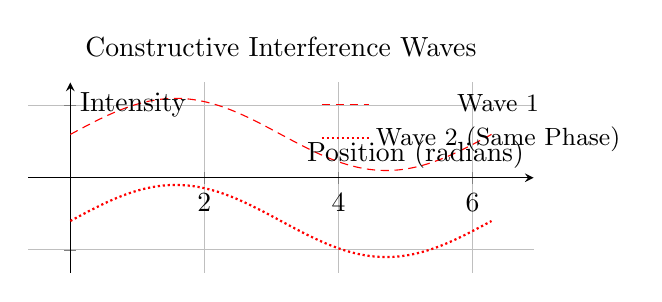
\begin{tikzpicture}
    \begin{axis}[
        title={Constructive Interference Waves},
        xlabel={Position (radians)},
        ylabel={Intensity},
        x label style={at={(axis description cs:1.05,-0.1)},anchor=north},
        yticklabel style={
            /pgf/number format/assume math mode, % This treats labels as math mode
            /pgf/number format/fixed zerofill,    % Adds zeros if needed for padding
            /pgf/number format/precision=1        % Precision of 1 for decimal places
        },
        ytick={},
        yticklabels={}, % Manually specify labels, leaving out -1 and 1
        domain=0:2*pi,
        samples=1000,
        axis lines=middle,
        enlargelimits,
        legend style={
            at={(1.2,1)}, 
            anchor=north east, 
            draw=none, 
            fill=none, 
            text opacity=1, 
            font=\small
        },
        height=4cm, width=8cm,
        grid=major
    ]
        % Wave 1
        \addplot[red, densely dashed] {0.5*sin(deg(x)) + 0.6};
        \addlegendentry{Wave 1}
        % Wave 2
        \addplot[red, densely dotted, thick] {0.5*sin(deg(x)) - 0.6};
        \addlegendentry{Wave 2 (Same Phase)}
        % Resultant Wave
        %\addplot[black] {0.5*sin(deg(x)) + 0.5*sin(deg(x))};
    \end{axis}
    \end{tikzpicture}
\end{minipage}
\hfill
\begin{minipage}{0.49\textwidth}
    \centering
    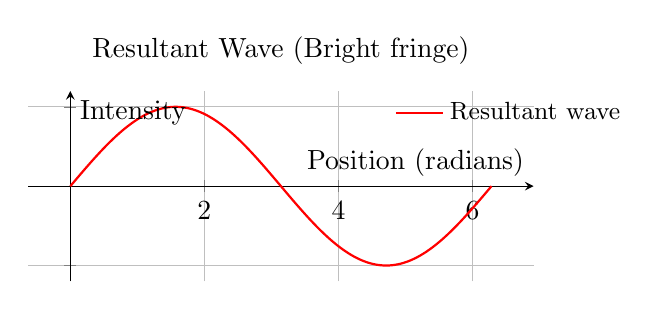
\begin{tikzpicture}
    \begin{axis}[
        title={Resultant Wave (Bright fringe)},
        xlabel={Position (radians)},
        ylabel={Intensity},
        x label style={at={(axis description cs:1.05,-0.1)},anchor=north},
        yticklabel style={
            /pgf/number format/assume math mode,
            /pgf/number format/fixed zerofill,
            /pgf/number format/precision=1
        },
        ytick={},
        yticklabels={},
        domain=0:2*pi,
        samples=1000,
        axis lines=middle,
        enlargelimits,
        height=4cm, width=8cm,
        grid=major,
        legend style={
            at={(1.2,1)}, 
            anchor=north east, 
            draw=none, 
            fill=none, 
            text opacity=1, 
            font=\small
        }
    ]
        % Resultant Wave
        \addplot[red, thick] {0.5*sin(deg(x)) + 0.5*sin(deg(x))};
        \addlegendentry{Resultant wave}
    \end{axis}
    \end{tikzpicture}
    \end{minipage}
\end{figure}

Destructive interference, on the other hand, occurs when the path difference is a half-integer multiple of the wavelength, resulting in dark fringes.\cite{enwiki:1212101911}

\begin{figure}[H]
    \centering
    \hfill
    \begin{minipage}{0.49\textwidth}
    \centering
    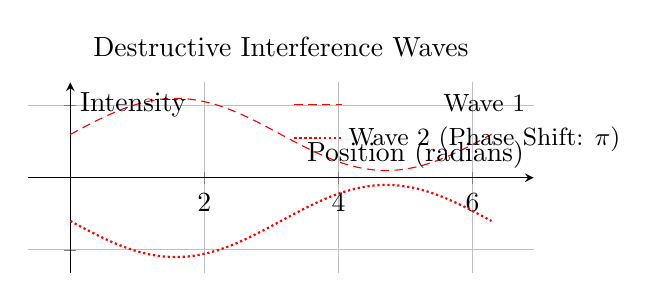
\begin{tikzpicture}
    \begin{axis}[
        title={Destructive Interference Waves},
        xlabel={Position (radians)},
        ylabel={Intensity},
        x label style={at={(axis description cs:1.05,-0.1)},anchor=north},
        yticklabel style={
            /pgf/number format/assume math mode,
            /pgf/number format/fixed zerofill,
            /pgf/number format/precision=1
        },
        ytick={},
        yticklabels={},
        domain=0:2*pi,
        samples=1000,
        axis lines=middle,
        enlargelimits,
        legend style={
            at={(1.2,1)}, 
            anchor=north east, 
            draw=none, 
            fill=none, 
            text opacity=1, 
            font=\small
        },
        height=4cm, width=8cm,
        grid=major
    ]
        % Wave 1
        \addplot[red, densely dashed] {0.5*sin(deg(x)) + 0.6};
        \addlegendentry{Wave 1}
        % Wave 3
        \addplot[red, densely dotted, thick] {0.5*sin(deg(x) + 180) - 0.6};
        \addlegendentry{Wave 2 (Phase Shift: $\pi$)}
    \end{axis}
    \end{tikzpicture}
    \end{minipage}
    \hfill
    \begin{minipage}{0.49\textwidth}
    \centering
    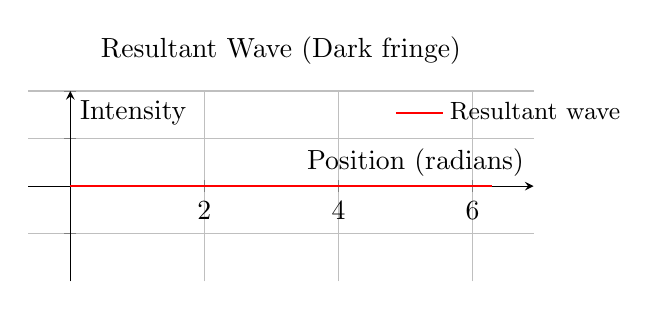
\begin{tikzpicture}
    \begin{axis}[
        title={Resultant Wave (Dark fringe)},
        xlabel={Position (radians)},
        ylabel={Intensity},
        x label style={at={(axis description cs:1.05,-0.1)},anchor=north},
        yticklabel style={
            /pgf/number format/assume math mode,
            /pgf/number format/fixed zerofill,
            /pgf/number format/precision=1
        },
        ytick={},
        yticklabels={},
        domain=0:2*pi,
        samples=1000,
        axis lines=middle,
        enlargelimits,
        height=4cm, width=8cm,
        grid=major,
        legend style={
            at={(1.2,1)}, 
            anchor=north east, 
            draw=none, 
            fill=none, 
            text opacity=1, 
            font=\small
        }
    ]
        % Resultant Wave (Destructive)
        \addplot[red, thick] {round(0.5*sin(deg(x)) + 0.5*sin(deg(x) + 180))};
        \addlegendentry{Resultant wave}
    \end{axis}
    \end{tikzpicture}
    \end{minipage}
\end{figure}


\subsubsection{Analysis of Fringe Patterns}
The pattern of the fringes provides information about the surface's properties:
\begin{itemize}
    \item \textbf{Straight and Parallel Fringes} indicate that the test surface is precisely flat. In this scenario, the fringes are parallel and uniformly spaced.
    \item \textbf{Curved Fringes} suggest that the surface is convex or concave. The curvature of the fringes gives clues about the curvature of the surface itself.
    \item \textbf{Irregular Fringes} are indicative of surface defects, bumps, or dips. The irregularity in spacing or the fringe shape can be analyzed to quantify the nature of the surface flaws.
\end{itemize}

\begin{frame}{}
    \begin{figure}[H]
    \centering
    \includegraphics[width=0.8\textwidth]{Images/Introduction/fringe_types}
    \caption{Different types of interference fringe patterns and what they indicate about surface characteristics.\cite{Joji_2023}}
    \label{fig:fringe-types}
    \end{figure}
\end{frame}

\section{Innovations in Optical Flat Technology}
\subsubsection{Plasmonic Optical Flat}
Recent advancements have expanded the traditional concept of optical flats to include plasmonic optical flats, which utilize nanostructured plasmonic surfaces. This innovation stems from the field of plasmonics, where the manipulation of light at the nanoscale allows for extreme localization and sensitivity to environmental changes. Plasmonic optical flats, comprised of nanostructured metal arrays, significantly enhance the sensitivity and resolution of surface inspections beyond the diffraction limit of light. These new optical flats are particularly effective in detecting sub-wavelength surface anomalies and offer the potential for rapid and precise surface inspection using simple, low-cost equipment.\cite{WOS:000387461800007}

\subsection{Phase Measuring Deflectometry}
A novel approach in the measurement of optical flats involves Phase Measuring Deflectometry (PMD), which offers a flexible and cost-effective alternative to interferometry. PMD uses a triangulation method involving a pinhole camera and LCD display to generate sinusoidal fringes, which are reflected by the flat surface. Distortions in these fringes are then captured and analyzed to determine the surface's figure. This technique is particularly advantageous for measuring surfaces where high slopes at edges or environmental sensitivities present challenges to traditional methods. The integration of PMD into optical flat metrology represents a significant shift towards more dynamic and accessible measurement technologies.\cite{WOS:000385319500019}

\section{Fringe Analysis in Optical Metrology}

Fringe analysis is an indispensable technique in the field of optical metrology, providing a non-intrusive means to capture and quantify physical phenomena with high precision. This method leverages the wave nature of light to generate fringe patterns, which are essentially contour maps representing variations in optical path length due to changes in physical properties like surface height, deformation, and refractive index changes.

The principle behind fringe analysis involves the interaction of light waves either through interference in interferometry or through projection in fringe projection techniques. In both instances, the resulting fringe patterns contain encoded information about the object's surface or the physical phenomenon being studied. The challenge, however, lies in converting these fringe patterns into quantitative data, a process that is achieved through various computational methods.

This chapter was mainly inspired by \texttt{Chapter 21: Fringe Analysis} in \texttt{Handbook of Optical Metrology by Toru Yoshizawa}\cite{fringe_analysis}

\subsection{Techniques in Fringe Analysis}
Two primary approaches define the landscape of fringe analysis:

\begin{enumerate}
    \item \textbf{Multiple-Input Image Techniques:} This approach utilizes multiple images of the fringe pattern, each obtained at a different phase shift. Common methods include the phase-shifting technique, where the phase of the reference beam is varied systematically to produce different fringe patterns, and the fringe scanning method, where the object or the fringe generator itself is moved to vary the fringe pattern.
    \item \textbf{Single-Input Image Techniques:} In scenarios where dynamic measurements are required, or it is impractical to obtain multiple images, single-input image techniques are employed. The Fourier Transform method is the most notable, using a single image with carrier fringes to extract phase information through spatial frequency analysis. We will elaborate more on this in the following section.
\end{enumerate}

\subsection{Fourier Transform Method}
The Fourier Transform (FT) method of fringe analysis represents a significant advancement in the field of optical metrology, particularly for dynamic measurements where the acquisition of multiple sequential images is impractical. This method, utilizing a single fringe image with carrier fringes, simplifies the setup and accelerates data processing, making it ideal for real-time applications.

\subsubsection{Principle of Operation}
The FT method involves the acquisition of a single fringe pattern that includes high-frequency carrier fringes. These carrier fringes are typically introduced by slightly tilting a reference beam in an interferometer setup, resulting in a fringe pattern with a well-defined spatial frequency. The mathematical basis of this approach is to model the intensity distribution of the fringe pattern as a sum of sinusoidal functions whose amplitudes encode the phase information of the surface being analyzed.

\begin{equation}
    I(x, y) = a(x, y) + b(x, y) \cos[2\pi f(x, y) + \phi(x, y)]
\end{equation}

Here, \( I(x, y) \) represents the recorded intensity, \( a(x, y) \) is the background illumination, \( b(x, y) \) denotes the amplitude of the modulation, \( f(x, y) \) is the carrier frequency, and \( \phi(x, y) \) is the phase to be recovered.

\subsubsection{Fourier Transform and Filtering}
The core step in the FT method is the Fourier transform of the recorded intensity distribution, which separates the frequency components. The high spatial frequency of the carrier fringes ensures their separation from the lower spatial frequency background. By filtering and isolating the frequency component corresponding to the carrier fringes, the phase information embedded in the fringes can be extracted effectively.

\begin{equation}
    \hat{I}(f_x, f_y) = \mathcal{F}\{I(x, y)\}
\end{equation}

Here, \( \hat{I}(f_x, f_y) \) represents the Fourier transform of the intensity distribution. Filtering around the carrier frequency \( f_0 \) isolates the relevant phase information.

\begin{frame}{}
    \begin{figure}[H]
        \centering
        \includegraphics[width=0.8\textwidth]{Images/Introduction/fourier_transform}
        \caption{1D Signal processing flow in FT method. This procedure can easily be extended to the 2D FT and filtering in a 2D frequency space.\cite{fringe_analysis}}
        \label{fig:fourier_transform}
    \end{figure}
\end{frame}

\subsubsection{Phase Demodulation and Reconstruction}
After filtering, the isolated component is shifted to zero frequency, and an inverse Fourier transform is applied to reconstruct the phase-modulated image. The phase at each point of the image can then be calculated using the arctan function applied to the real and imaginary parts of the reconstructed image.

\begin{equation}
    \phi(x, y) = \arctan\left(\frac{\text{Im}[\mathcal{F}^{-1}(\hat{I}(f_x, f_y))]}{\text{Re}[\mathcal{F}^{-1}(\hat{I}(f_x, f_y))]}\right)
\end{equation}

This reconstructed phase map provides a direct measurement of the optical path differences induced by the object's surface, translating physical deformations into measurable phase shifts.

\subsubsection{Rationale for Using the Fourier Transform Method}
The adoption of the Fourier Transform (FT) method in fringe analysis is driven by several practical and academic motivations, particularly suited to scenarios where obtaining multiple images with varied fringe patterns is challenging. One such scenario is when using an optical flat, which typically produces only one image. The inherent difficulty in capturing multiple images with different fringe patterns at the exact same position makes the FT method highly valuable. This method can extract detailed phase information from a single static image, circumventing the need for moving the setup to introduce different phase shifts, which is often impractical or impossible with an optical flat.

Additionally, my interest in applying signal processing techniques beyond theoretical mathematics classes has led me to explore the use of Fourier Transform in a practical, real-world application. The FT method offers a profound application of Fourier analysis, allowing the decomposition of an image into its frequency components. This not only aids in isolating the phase information crucial for metrological assessments but also reinforces the foundational signal processing principles by applying them to solve complex engineering problems.

\subsection{Phase Unwrapping}
Phase unwrapping is an essential process in fringe analysis, addressing the intrinsic limitation where phase measurements are typically confined within a $[-\pi, \pi]$ interval, known as phase wrapping. This phenomenon occurs because the phase response of the imaging system is cyclic, with each cycle representing a change in phase of $2\pi$. Hence, any phase change beyond this range results in a modulo $2\pi$ calculation, which can obscure the true phase changes caused by the physical properties of the object being studied.

\begin{frame}{}
    \begin{figure}[H]
        \centering
        \includegraphics[width=0.8\textwidth]{Images/Introduction/phase_unwrapping}
        \caption{Phase unwrapping.\cite{fringe_analysis}}
        \label{fig:phase_wrapping}
    \end{figure}
\end{frame}

\subsubsection{Challenges of Phase Wrapping}
In practical applications, such as 3D surface profiling or deformation analysis, this wrapping effect can create discontinuities in the computed phase map, appearing as abrupt jumps from $-\pi$ to $\pi$ and vice versa. These discontinuities can significantly distort the resulting measurements, making it impossible to directly infer the true topographical features of the surface under investigation without additional processing.

\subsubsection{Unwrapping Algorithms}
Phase unwrapping seeks to mitigate these issues by reconstructing the original phase distribution that extends beyond the $[-\pi, \pi]$ range. The process involves algorithmically adding or subtracting $2\pi$ where necessary to eliminate the discontinuities, thereby 'unwrapping' the phase to reflect the true surface characteristics.

\subsubsection{Simple Phase Unwrapping Using Adjacent Pixel Comparison}
In the most straightforward cases of phase unwrapping, the goal is to correct phase discontinuities along a specified path, typically one-dimensional, across the image. This method involves comparing the phase values of adjacent pixels and making corrections when abrupt changes are detected that indicate wrapping. The process is governed by the following set of rules:

\begin{equation}
    \phi_{\text{unwrapped}}(i) = 
    \begin{cases} 
    \phi(i) - 2\pi & \text{if } \phi(i) - \phi(i-1) > \pi \\
    \phi(i) + 2\pi & \text{if } \phi(i) - \phi(i-1) < -\pi \\
    \phi(i) & \text{otherwise}
    \end{cases}
\end{equation}

where \( \phi(i) \) is the wrapped phase at pixel \( i \) and \( \phi_{\text{unwrapped}}(i) \) is the corrected phase value. This method assumes a sequential progression through the image pixels, typically from left to right or top to bottom.

Phase unwrapping can be particularly challenging in scenarios where fringe patterns are surrounded by nonrectangular boundaries or contain singular points—locations where the fringe modulation is very low or the phase differences exceed \(2\pi\). In such cases, the phase unwrapping path may be accidentally interrupted, leading to deviations from the true phase distribution. To address these complexities, several robust algorithms have been developed:

\begin{itemize}
    \item \textbf{Minimum-Spanning Tree (MST) Algorithms:} These methods create a continuous phase-unwrapping path by spanning the effective phase area with tree-like trajectories. They are designed to avoid creating localized loops and use cost functions such as the spatial phase gradient and fringe contrast to assess and ensure the reliability of the pixels. Unreliable pixels are identified and removed from the spanning tree, facilitating a smoother unwrapping process.
    \item \textbf{Energy Minimization Algorithms:} This approach involves minimizing an energy function that quantifies the discontinuities in the phase map. The algorithm iteratively adjusts the phases by \( \pm 2\pi \) to reduce the total energy, aiming for a state where the sum of squared differences of neighboring pixels is minimized. This method is particularly effective as it does not rely on a predefined path and can adapt to the local characteristics of the phase data.
    \item \textbf{Error Correction and Singular Point Handling:} Before unwrapping, it is crucial to identify and address singular points where errors are likely due to low modulation or high noise. Techniques include using local operations to assess the consistency of the phase differences around these points. If necessary, lines connecting points of opposite discontinuity signs are established as boundaries not to be crossed during the unwrapping process.
\end{itemize}


\end{document}
